% \clearpage
% \begin{subappendices}
\newappendix{Grid-world visualizations} \label{sec:gridworld-vis}

The grid-world environment we use consists of a 40x40 environment with actions up, down, left, and right, with a single start state in the lower left and a single goal state in the upper right.
In \Cref{fig:gridworld_algorithm_states} we show the state of each algorithm after training on the grid-world for 100 episodes.
While DDQN and BBE have only visited a small fraction of the states, \algshort{} has covered most of the environment and will soon solve it.
As they continue to run BBE will eventually find the goal while DDQN will not.

A video version of \Cref{fig:gridworld_algorithm_states}, which shows its evolution over time, is available in the supplement.
We find that watching the qualitative behavior of each algorithm can be enlightening.
Note that as the figures and videos are rendered by sampling states and actions, some noise in the form of missing states may appear.

\begin{figure}[h]
    \centering
    \begin{subfigure}[b]{\textwidth}
        \centering
        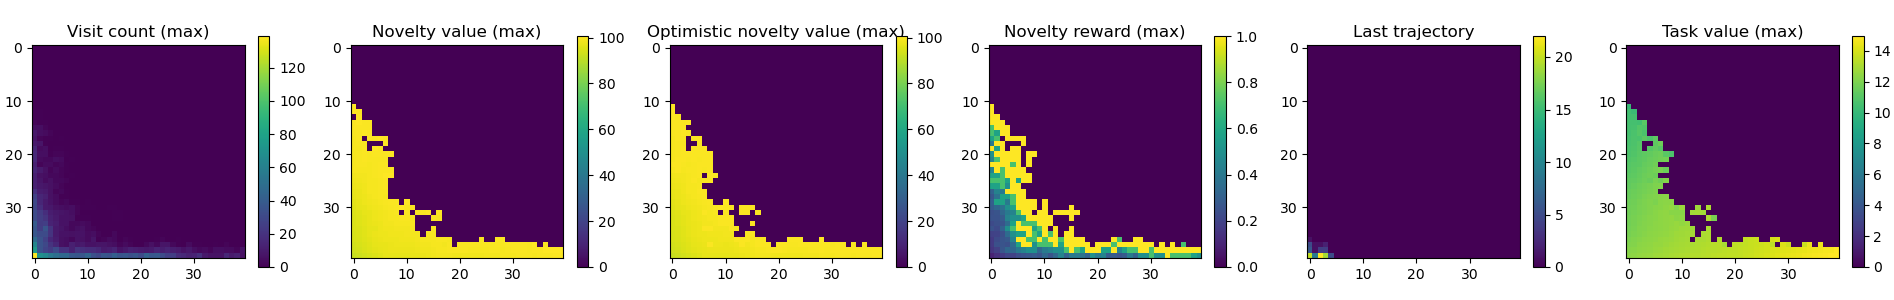
\includegraphics[height=0.15\textwidth]{figures/deep/gridworld_100_ddqn.png}
        \caption{DDQN}
    \end{subfigure}

    \begin{subfigure}[b]{\textwidth}
        \centering
        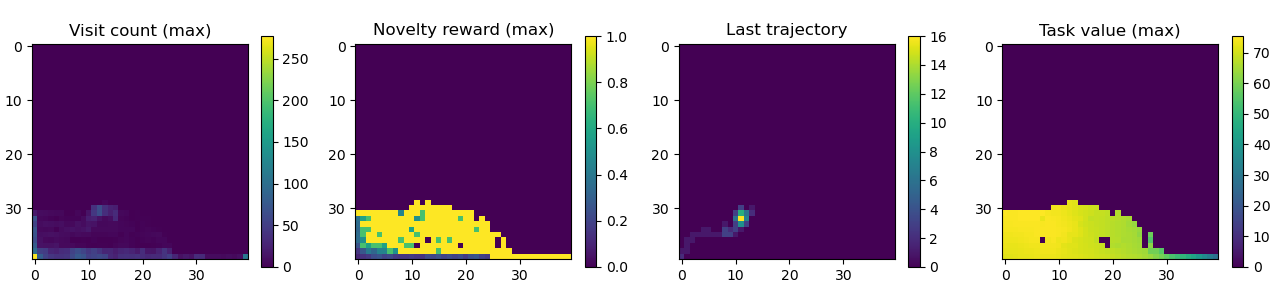
\includegraphics[height=0.15\textwidth]{figures/deep/gridworld_100_bbe.png}
        \caption{BBE}
    \end{subfigure}

    \begin{subfigure}[b]{\textwidth}
        \centering
        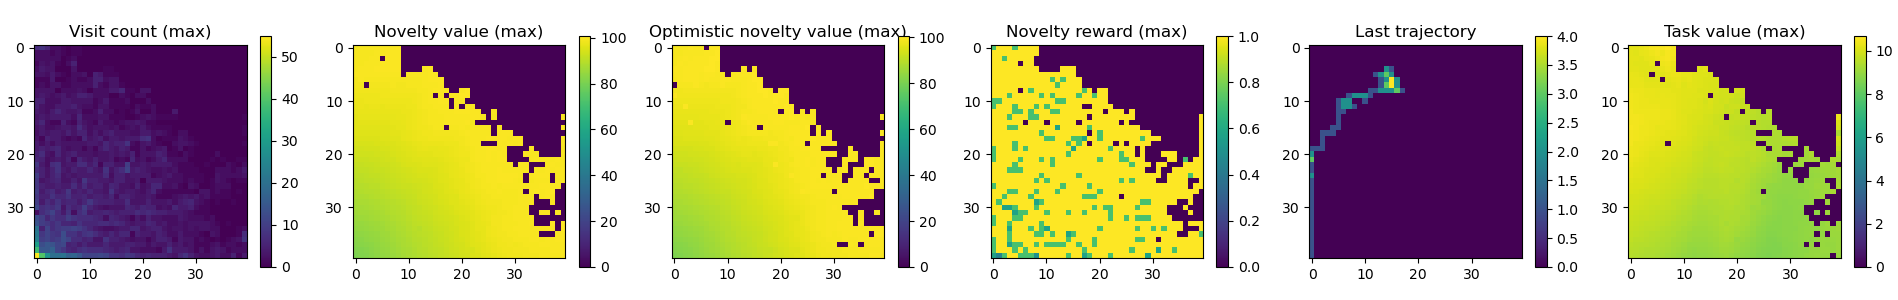
\includegraphics[height=0.15\textwidth]{figures/deep/gridworld_100_deep.png}
        \caption{DEEP}
    \end{subfigure}
    \caption{The state of each algorithm after 100 episodes in the grid-world environment.
        Note that the novelty reward and novelty value shown for DDQN are for visualization purposes only, as the algorithm does not use them.
        The ``Task value'' shown for BBE is the sum of the task and novelty rewards, which BBE treats as its objective.
        Un-visited states are marked as zero in each plot.
        The annotation (max) indicates that the value shown is the maximum value for any action at that state.
        ``Last trajectory'' shows the states visited in the last training episode.
        Figures generated by sampling.}
        \label{fig:gridworld_algorithm_states}
\end{figure}


\newappendix{Pseudo-count implementation} \label{sec:count_implementation}

% Our implementation of the kernel-based pseudo-count described in \Cref{sec:kernel_counts} has two

Define the Gaussian kernel with dimension $d$ as
\begin{align}
    k_\text{Gauss}(x, x_i) = (2 \pi) ^ {-\frac{d}{2}} \det(\bm{\Sigma})^{-\frac{1}{2}} \exp \left\{-\frac{1}{2} (x - x_i)^\intercal \bm{\Sigma}^{-1} (x - x_i) \right\}.
\end{align}
We can normalize this function to have a maximum at $k(x, x) = 1$ simply by removing the normalizer (everything outside the exponential) by noting that $e^0 = 1$.
This gives the kernel we use:
\begin{align} \label{eq:count_kernel}
    k(x, x_i) = \exp \left\{-\frac{1}{2} (x - x_i)^\intercal \bm{\Sigma}^{-1} (x - x_i) \right\},
\end{align}
where the covariance is a diagonal matrix $\bm{\Sigma} = \text{diag}(\sigma_1^2, \ldots, \sigma_d^2)$.

To compute $\hat N_n(s, a)$ using this kernel, we perform the following steps:
\begin{enumerate}
    \item Normalize $s$ and $a$:
    \begin{align}
        \bar{s} = \frac{s - \mathcal{S}_\text{min}}{\mathcal{S}_\text{max} - \mathcal{S}_\text{min}} && \bar{a} = \frac{a - \mathcal{A}_\text{min}}{\mathcal{A}_\text{max} - \mathcal{A}_\text{min}}
    \end{align}
    \item Define $x = [\bar{s}, \bar{a}]$ as the concatenation of the normalized state and action.
    \item Compute the kernel from \cref{eq:count_kernel} and sum across all of the previous normalized observations $x_i$:
    \begin{align}
        \hat N_n(s, a) = \hat N_n(x) = \sum_{i=1}^n k(x, x_i)
    \end{align}
\end{enumerate}

For this final step, we leverage the MIT-licensed Kernel Operations library (KeOps, \citet{keops}), a high-performance GPU-accelerated library for efficient computation of reductions on symbolically-defined matrices.
This substantially outperforms implementations in other frameworks, including fully-JITted JAX \citep{jax2018github} version, especially as the dimension of the data grows.

To avoid having to tune the covariance for each environment, we adapt the scaling rule of \citep{Henderson2012NormalRB}.
This rule of thumb requires assumptions on the data (notably, that it comes i.i.d. from a Normal) which are violated in the exploration problem.
However, we find this scaling to be useful in practice.
The rule of thumb bandwidth for dimension $j$ of the data for a multivariate Gaussian kernel is
\begin{align}
    h_j^{ROT} = \left( \frac{4}{2+d}  \right) ^ \frac{1}{4+d} \hat{\sigma}_j n ^ {- \frac{1}{4+d}},
\end{align}
where $\hat{\sigma}_j$ is the empirical variance of dimension $j$ of the data.
Making the assumption that our states are normalized to be in $[-1, 1]$ and distributed uniformly, we can set $\hat{\sigma}_j \approx 0.3$.
As such, in every experiment with continuous-valued states, we set the kernel variance for dimension $j$ as
\begin{align}
    \sigma_j = 0.3 \left( \frac{4}{2+d} \right) ^ \frac{1}{4+d} n ^ {- \frac{1}{4+d}} .
\end{align}
In experiments we find that changes to this scale of less than an order of magnitude make little difference.

Throughout we use 1 for the kernel variance on the action dimensions.

\subsection{Updating the kernel estimator}
Updates to the kernel count estimator consist of appending new normalized observations to the set $\{x_i\}$.
However, we find that computing this kernel becomes prohibitively slow beyond roughly 100K entries, and our experiments run for up to 1M steps.
We take two steps to avoid this slowdown.
Both rely on nonuniform weighting of entries in the observation table when computing the count, leading us to maintain an additional array of weights in addition to the table of observations.

\paragraph{Avoiding duplicate entries.}
If a new observation $x$ has $k(x, x_i) > 0.95$ with some set $M$ of existing indices, we do not add $x$ to the table, and instead add $\nicefrac{1}{|M|}$ to each entry $i \in M$ of the weights table.
In essence, if there is an exact duplicate for $x$ in the table already, we simply count that existing entry twice.
While this is helpful, the probability of observing exact matches decreases rapidly in the dimension of the observations, so this step plays a limited role.

\paragraph{Evicting previous entries.}
Once the length of the observations table reaches some maximum ($2^{15} = 32768$ in our experiments), we evict an existing entry in the table uniformly at random when we make a new entry, thus maintaining the table at that maximum size.
This introduces risk that the exploration bonus would not go to zero in the limit of many environment steps, which we avoid by re-distributing the weight of the evicted observations among those still in the table.
We do this redistribution uniformly; that is, if we evict the entry at location $i$, with weight $w_i$, we add $w_i / (n-1)$ to the weight of each of the $(n-1)$ other entries.
Our reweighting procedure maintains the same \emph{total} amount of count when evicting observations and ensures that bonuses go to zero in the limit of data.
In experiments we find that the exploration rewards earned when using a very small observation table (and thus, many evictions) were practically indistinguishable from using an observation table of unlimited size.


\subsection{Tabular environments}
For the grid-world environment used in \Cref{fig:gridworld_warmstart,fig:gridworld_visits}, we use a tabular visit count rather than pseudo-counts.


\newappendix{Details on rapid Q updates} \label{sec:fast_updates_appendix}

We aim to rapidly update $\qex$ to maximize reward on the non-stationary exploration MDP $\mdp_{R^+_n}$ and thus explore rapidly.
This has three components: (1) updating using the current reward function $R^+_n$ rather than logged rewards, (2) performing many updates to $\qex$ at every timestep using a large learning rate, and (3) using an optimistic version of $\qex$ which is aware of the high value of taking actions that have not yet been explored.
However, aggressively updating $\qex$ poses its own problems; most significantly, Q-learning with function approximation has a tendency to diverge if updated too aggressively with too few new samples.
We use three modifications to the typical Bellman update with target networks \citep{mnih2015human} to mitigate this issue while incorporating optimism.

\begin{itemize}
    \item \textbf{Soft DoubleDQN update.} The DoubleDQN \citep{Hasselt2016DeepRL} update reduces overestimation in Q-learning by selecting and evaluating actions using different parameters.
    We use a soft version of the DoubleDQN update by replacing the max operator with an exponential-Q policy over uniform random actions using a low temperature.
    \item \textbf{Value clipping.} To further mitigate the problem of Q-learning overestimation and divergence, we clip the Bellman targets to be within the range of possible Q values for $\mdp_{R^+_n}$.
    Given that the rewards $r^+$ are scaled to be in $[0, 1]$, any policy would have a value $\qex(s, a) \in [0, \bar{r}]$, where $\bar{r} = \nicefrac{1}{1 - \gamma}$.
    \item \textbf{Optimistic targets.} We use the optimistic adjustment in \cref{eq:optimism} when computing targets.
\end{itemize}

Define the softmax-Q policy for some Q function $Q$ as
\begin{align}
    \pi(a \mid s; Q) = \frac{\exp \big\{ \nicefrac{Q(s, a)}{\tau} \big\}}{\int_\mathcal{A} \exp \big\{ \nicefrac{Q(s, a')}{\tau}  ~da' \big\}}
\end{align}
which we approximate using self-normalized importance sampling with a uniform proposal distribution.
The target for updating $\qex$ is
\begin{align} \label{eq:update_target}
    y(s, a, s') = \text{clip} \left( R^+_n(s, a) + \gamma \E_{a' \sim \pi(\cdot \mid s'; \qex^+)} \Big[ \qex^+(s', a'; \theta^-) \Big], 0, \bar{r} \right).
\end{align}
where $R^+_n(s, a)$ is the current exploration bonus, which we recompute at update time; $\qex^+(s', a'; \theta^-)$ is the target network for the exploration value function, with optimism applied.
We then minimize the squared error between $y(s, a, s')$ and $\qex(s, a)$.


\newappendix{Environments for exploration} \label{sec:environments_appendix}

To enable benchmarking the performance of exploration methods on continuous control, we constructed a new set of environments.
Our motivation comes from the challenges of performing resets and defining shaped rewards in real-world robotics, where it is not possible to measure and set states exactly.
Unlike in simulation, it may be difficult or impossible to implement uniform resets of the robot and the objects in the scene; states with a walking robot standing upright or a block in midair require significant expertise to reach.
Similarly many shaped rewards in simulation rely on precise knowledge of the locations of objects in a scene to provide rewards corresponding to e.g. an objects distance from a goal.
We make modifications which capture the spirit of these real-world constraints, though these exact environments might still be difficult to construct in the real world:
\begin{itemize}
    \item Small reset distributions.
    Instead of resetting every object in the scene uniformly in the space, we randomize each object's configuration over a smaller set of starting states.
    This reflects some properties of real environments, such as walking robots starting on the ground instead of midair, or the object in a manipulation task not starting in its goal receptacle.
    \item Sparse rewards.
    While dense rewards are difficult to construct without real-time monitoring of object positions, sparse rewards are often simpler.
    A picking task, for example, can provide a sparse reward simply by checking whether the desired object is inside a receptacle.
\end{itemize}

As the base environments for our benchmark, we select four tasks from DeepMind Control Suite \citep{tassa2018deepmind}, an Apache-licensed standard set of benchmarks implemented using the commercial MuJoCo physics simulator \citep{todorov2012mujoco}.
Denoting the state (observation) and action dimensions of an environment as $\text{dim}(\mathcal{S}) \rightarrow \text{dim}(\mathcal{A})$, these environments are:
\begin{itemize}
    \item \textbf{Ball-in-cup catch} (manipulation, $8d \rightarrow 2d$).
    \item \textbf{Reacher hard} (goal-directed, $6d \rightarrow 2d$).
    \item \textbf{Finger turn\_hard} (manipulation, goal-directed, $12d \rightarrow 2d$).
    \item \textbf{Walker walk} (locomotion, $24d \rightarrow 6d$).
\end{itemize}

We modify each environment to remove the accommodations of wide reset distributions and sparse rewards which make them easy to solve without directed exploration.
The new environments and their changes are as follows:
\begin{itemize}
    \item \textbf{Ball-in-cup explore} (manipulation, $8d \rightarrow 2d$). The original task resets the ball uniformly in the reachable space, including already in the cup (the goal state).
    We modify the environment to only reset the ball in a region below the cup, as if the ball was hanging and gently swinging.
    The original task already has sparse rewards.
    \item \textbf{Reacher explore} (goal-directed, $6d \rightarrow 2d$).
    The original task samples arm positions and goal positions uniformly, resulting in the arm being reset very near the goal.
    We modify the reset distribution to only include states with the arm mostly extended to the right and targets opposite it on the left in a cone with angle $\pi/2$.
    Note that this task is somewhat easier than the original since the policy only needs to navigate between smaller regions of the space, but is harder due to the resets not providing exploration.
    The original task already has sparse rewards.
    \item \textbf{Finger explore} (manipulation, goal-directed, $12d \rightarrow 2d$).
    The original task resets the finger uniformly, the angle of the spinner uniformly, and the goal location uniformly on the circle reachable by the tip of the spinner.
    We modify the environment to reset the finger joints each in the quadrant pointing away from the spinner, the spinner pointing in the downward quadrant, and the target in the upward quadrant.
    Similarly to Reacher explore, this task is simpler than the original but harder to explore in.
    The original task already has sparse rewards.
    \item \textbf{Walker explore} (locomotion, $24d \rightarrow 6d$).
    The original environment resets the walker just above the ground with random joint angles, leading to it frequently starting upright and in position to begin walking.
    We modify the environment by allowing time to progress for 200 steps in the underlying physics (20 environment steps), which is enough time for the walker to fall to the floor.
    This simulates the walker starting in a random lying-down configuration.
    The original rewards include a sparse reward for being upright and above a certain height and a linear component for forward velocity.
    We replace the forward velocity reward with a sparse version which provides reward only when the agent is moving at or above the target speed.
\end{itemize}

The code for these environments is included in the supplement.



\newappendix{Experimental implementation details} \label{sec:appendix_benchmark_implementation}

\subsection{Computing infrastructure}
We implemented \algshort{} using JAX \citep{jax2018github} and the neural network library Flax \citep{flax2020github} which is built on it, both of which are Apache-licensed libraries released by Google.
The SAC implementation we use is from \citet{pytorch_sac} (MIT-licensed), built on Pytorch \citep{Paszke2019PyTorchAI} (custom BSD-style license).
The experiments in this paper take about a week to run using 16 late-model NVidia GPUs by running 2-4 seeds of each experiment at once on each GPU.

\subsection{Network architectures and training}
For the Q networks used as $\qex$ in continuous environments and as the task policy in the grid-world experiments, we use fully-connected networks with two hidden layers of 512 units each and ReLU activations.
These networks flatten and concatenate the state and action together to use as input and produce a 1d value prediction.
This enables us to use the same networks and training for discrete and continuous actions rather than using the usual discrete-action trick of simultaneously producing a Q-value estimate for every action given the state.

These Q networks are trained using the Adam optimizer \citep{kingma2014adam} with learning rate $10^{-3}$.
$\qex$ is updated with two Bellman updates with batch size 128 per environment step.
We update the target network after every environment step for $\qex$ to allow very rapid information propagation about changing rewards.
For the Q network defining $\pitask$ in the grid-world we use a learning rate of $10^{-4}$ and update the target network after every 50 Bellman updates.

\subsection{Other hyperparameters}
We draw 64 samples from $\pitask$ when computing the behavior policy and 64 samples from a uniform distribution over actions when updating $\qex$ as described in Appendix \Cref{sec:fast_updates_appendix}.
We set the temperature for Boltzmann sampling from all Q-network policies as $\tau = 0.1$.
$\qex$ uses a discount $\gamma = 0.99$.


% \newpage
\newappendix{Additional benchmark results} \label{sec:benchmark_results_appendix}

We performed an experiment to check whether it was simply the separation of learning two separate Q functions which enabled \algshort{}'s performance.
To do this, we modified SAC + BBE to learn one Q function for the task reward function and one Q function for the exploration reward function.
The policy was then trained to maximize the sum of those two Q functions.
This baseline, which we call SAC 2Q, performed uniformly worse than SAC + BBE, but we include its results here for completeness.


\begin{figure}[h]
    \centering
    \begin{subfigure}[b]{0.24\textwidth}
        \centering
        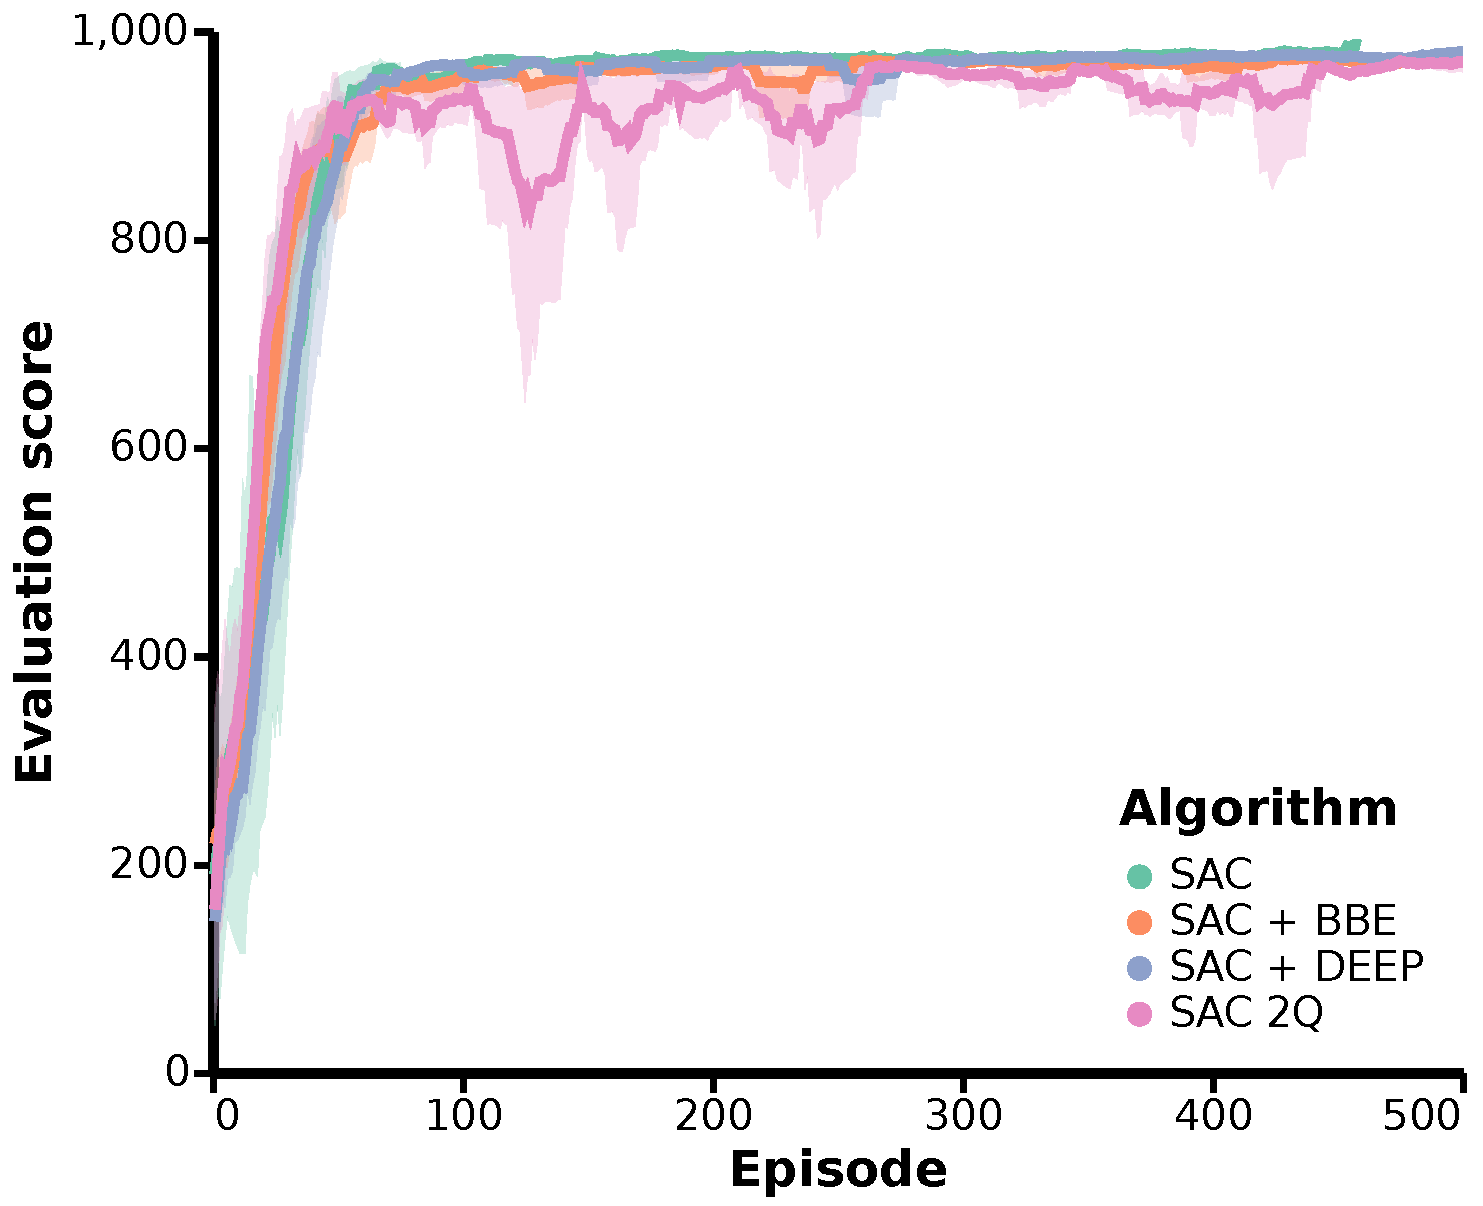
\includegraphics[width=\textwidth]{figures/deep/neurips_SAC2Q_ball_in_cup.pdf}
        \caption{Ball-in-cup}
    \end{subfigure}
    \begin{subfigure}[b]{0.24\textwidth}
        \centering
        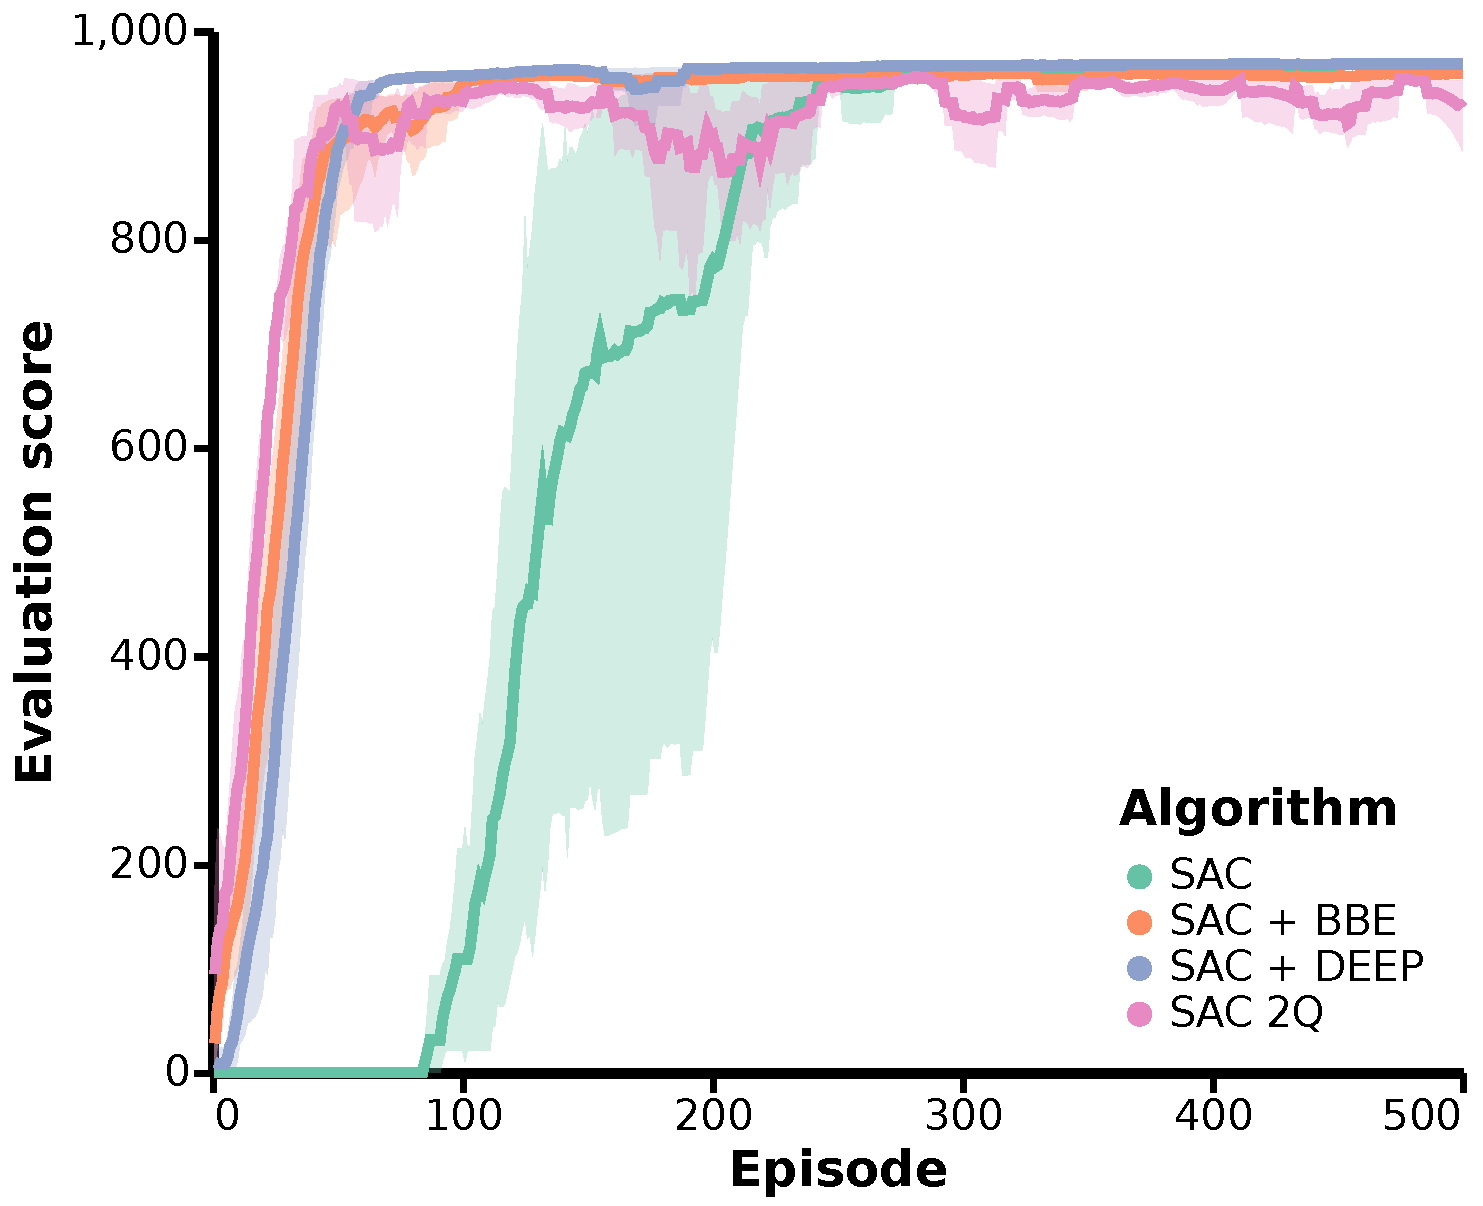
\includegraphics[width=\textwidth]{figures/deep/neurips_SAC2Q_ball_in_cup_explore.pdf}
        \caption{Ball-in-cup explore}
    \end{subfigure}
    \hfill
    \begin{subfigure}[b]{0.24\textwidth}
        \centering
        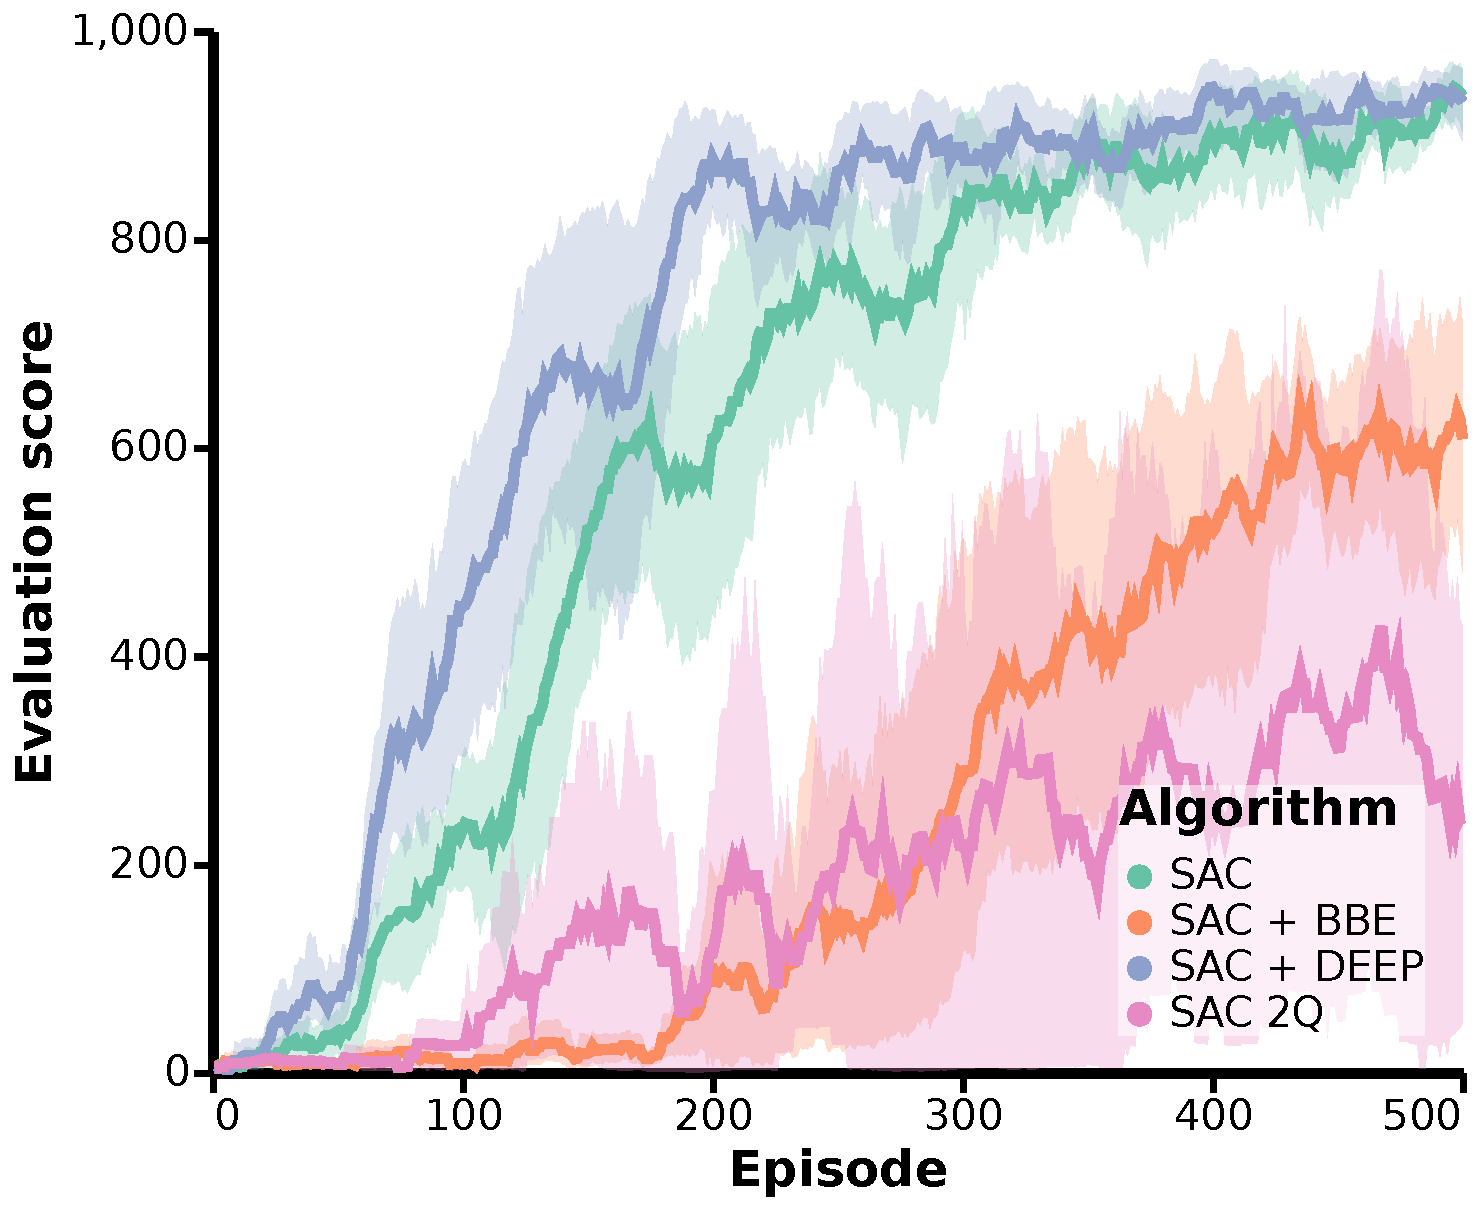
\includegraphics[width=\textwidth]{figures/deep/neurips_SAC2Q_reacher.pdf}
        \caption{Reacher}
    \end{subfigure}
    \begin{subfigure}[b]{0.24\textwidth}
        \centering
        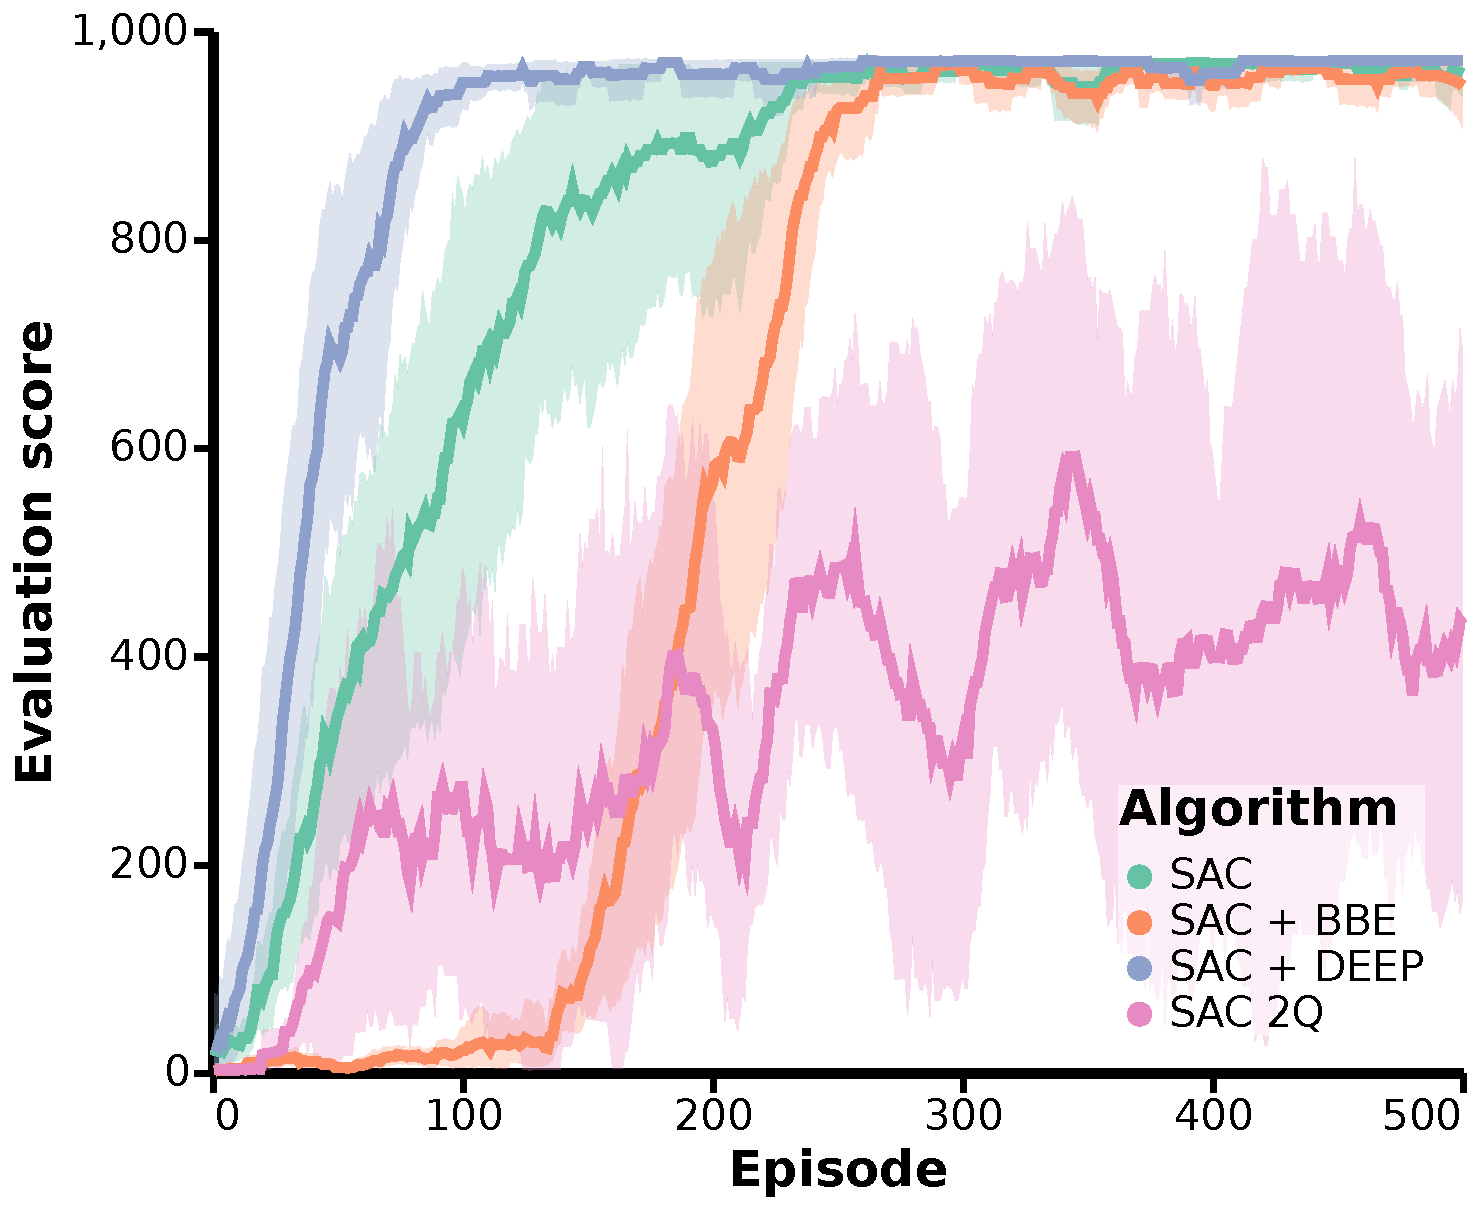
\includegraphics[width=\textwidth]{figures/deep/neurips_SAC2Q_reacher_explore.pdf}
        \caption{Reacher explore}
    \end{subfigure}
    \vspace{1em}

    \begin{subfigure}[b]{0.24\textwidth}
        \centering
        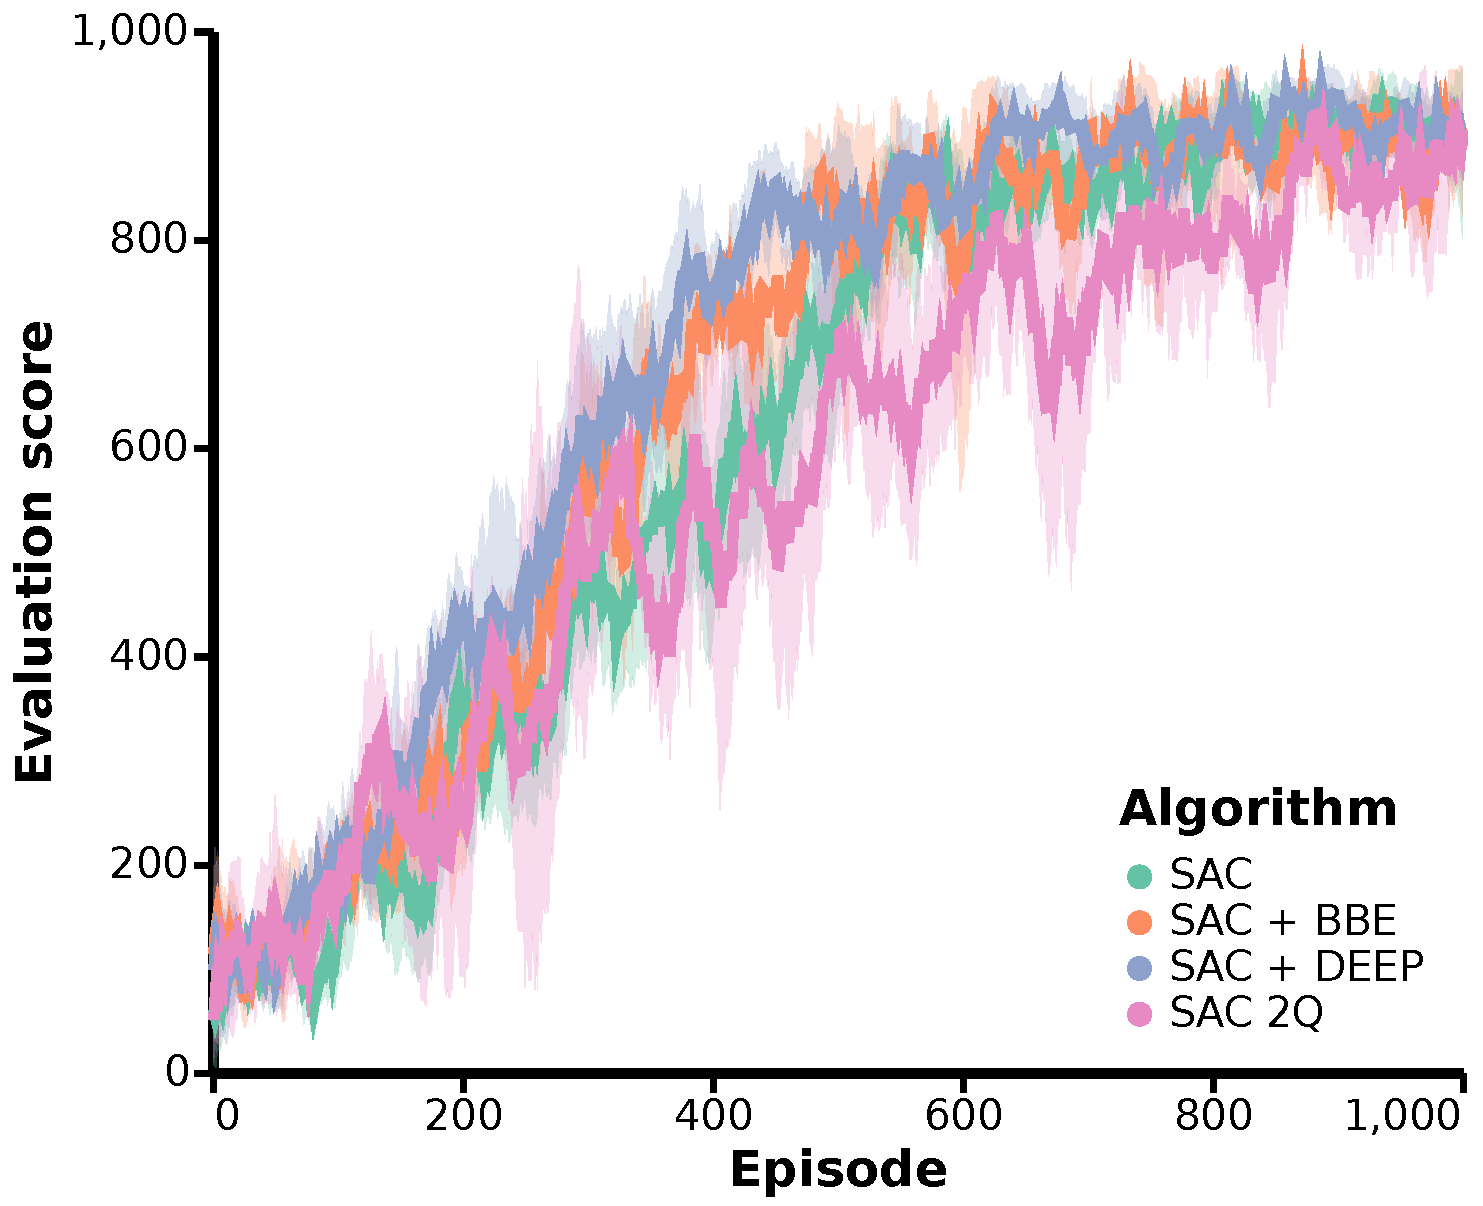
\includegraphics[width=\textwidth]{figures/deep/neurips_SAC2Q_finger.pdf}
        \caption{Finger}
    \end{subfigure}
    \begin{subfigure}[b]{0.24\textwidth}
        \centering
        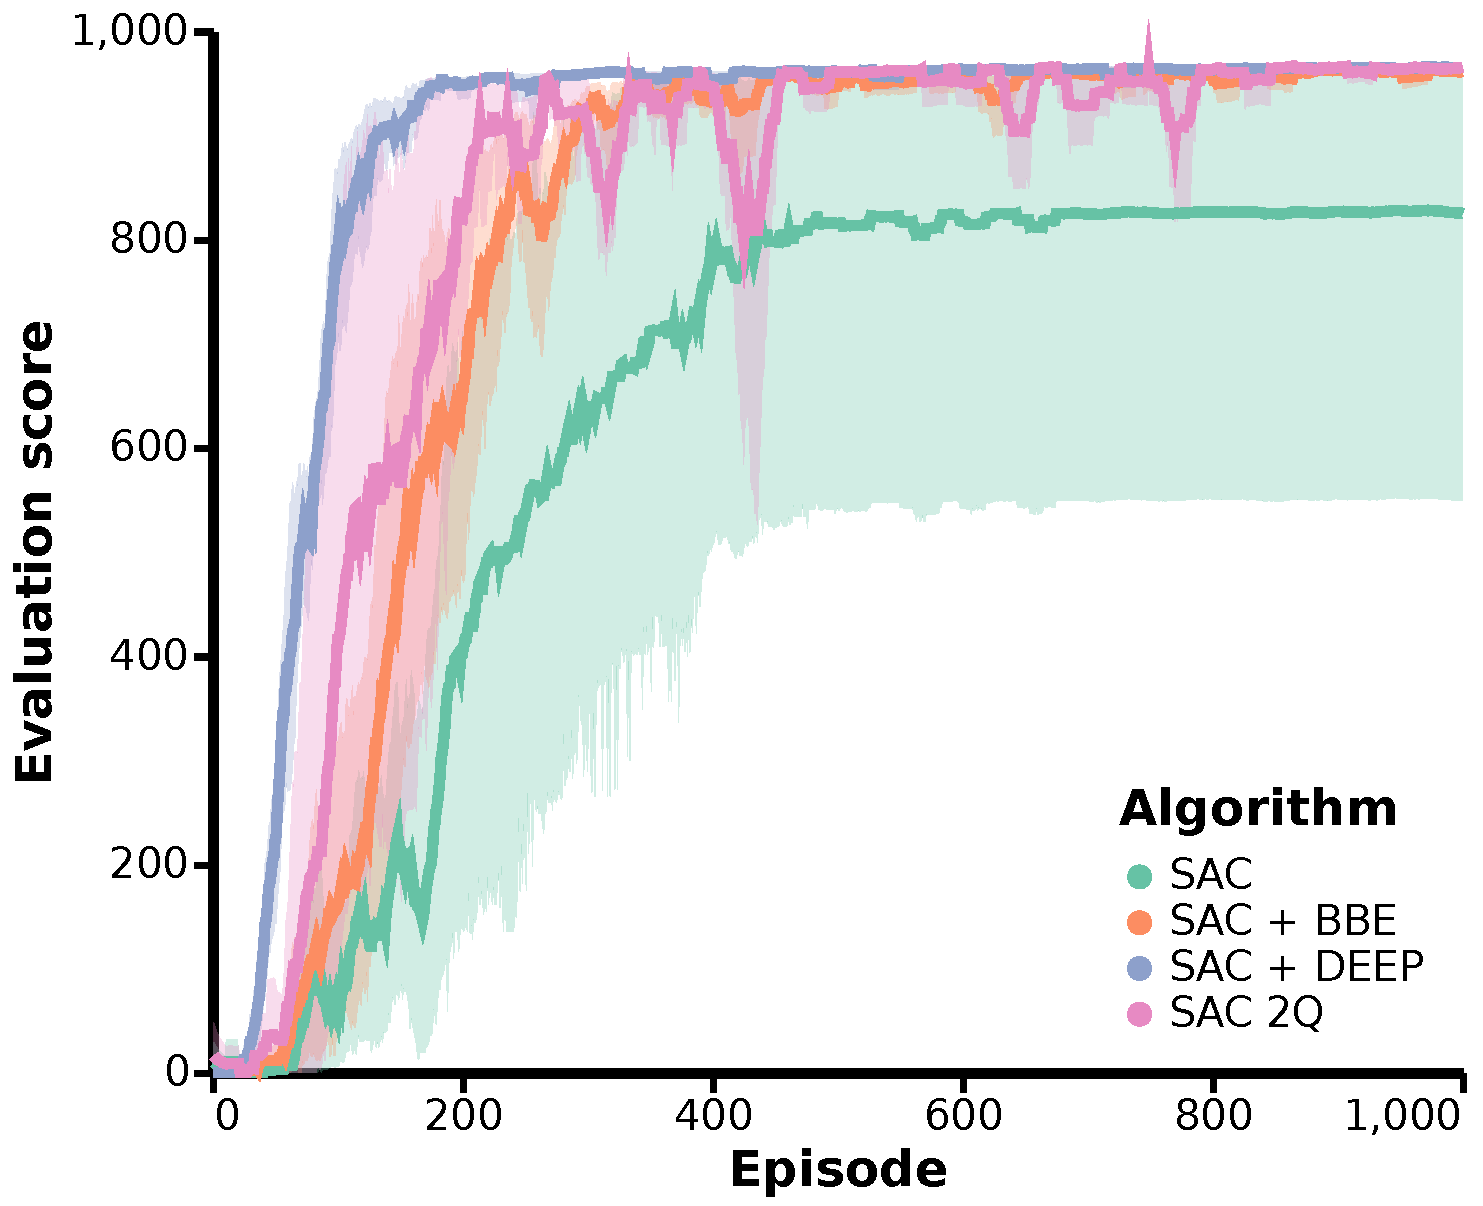
\includegraphics[width=\textwidth]{figures/deep/neurips_SAC2Q_finger_explore.pdf}
        \caption{Finger explore}
    \end{subfigure}
    \hfill
    \begin{subfigure}[b]{0.24\textwidth}
        \centering
        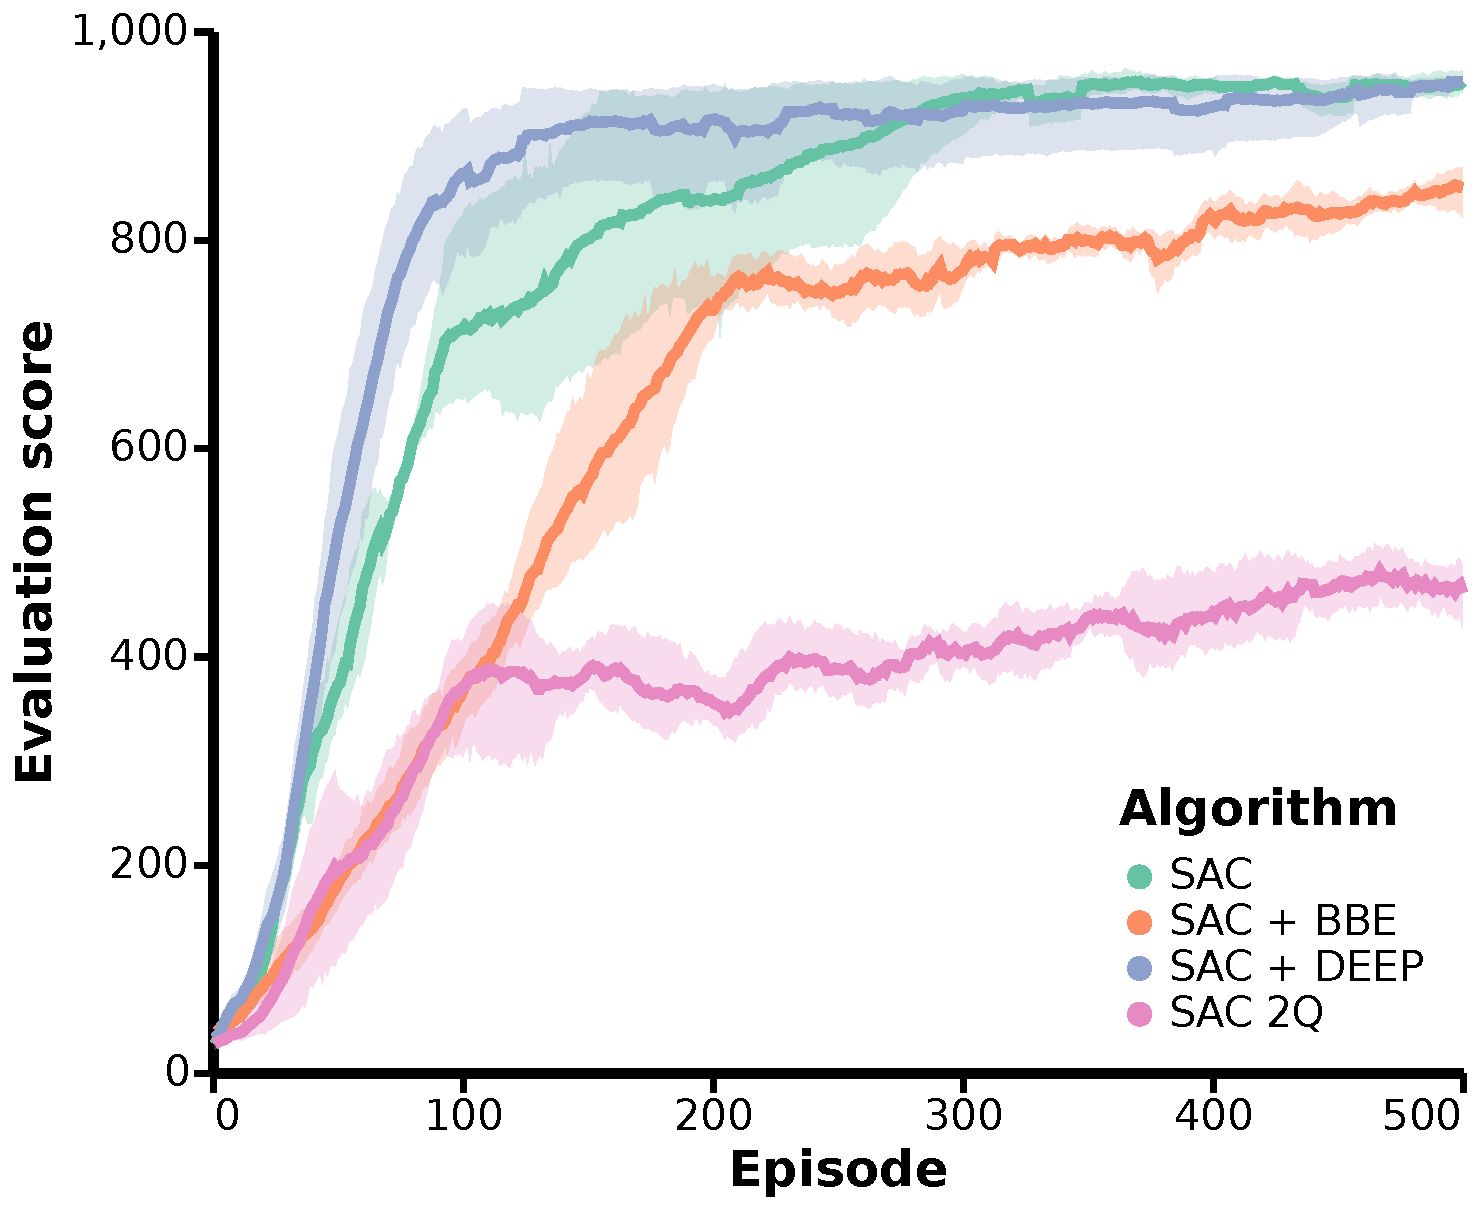
\includegraphics[width=\textwidth]{figures/deep/neurips_SAC2Q_walker.pdf}
        \caption{Walker}
    \end{subfigure}
    \begin{subfigure}[b]{0.24\textwidth}
        \centering
        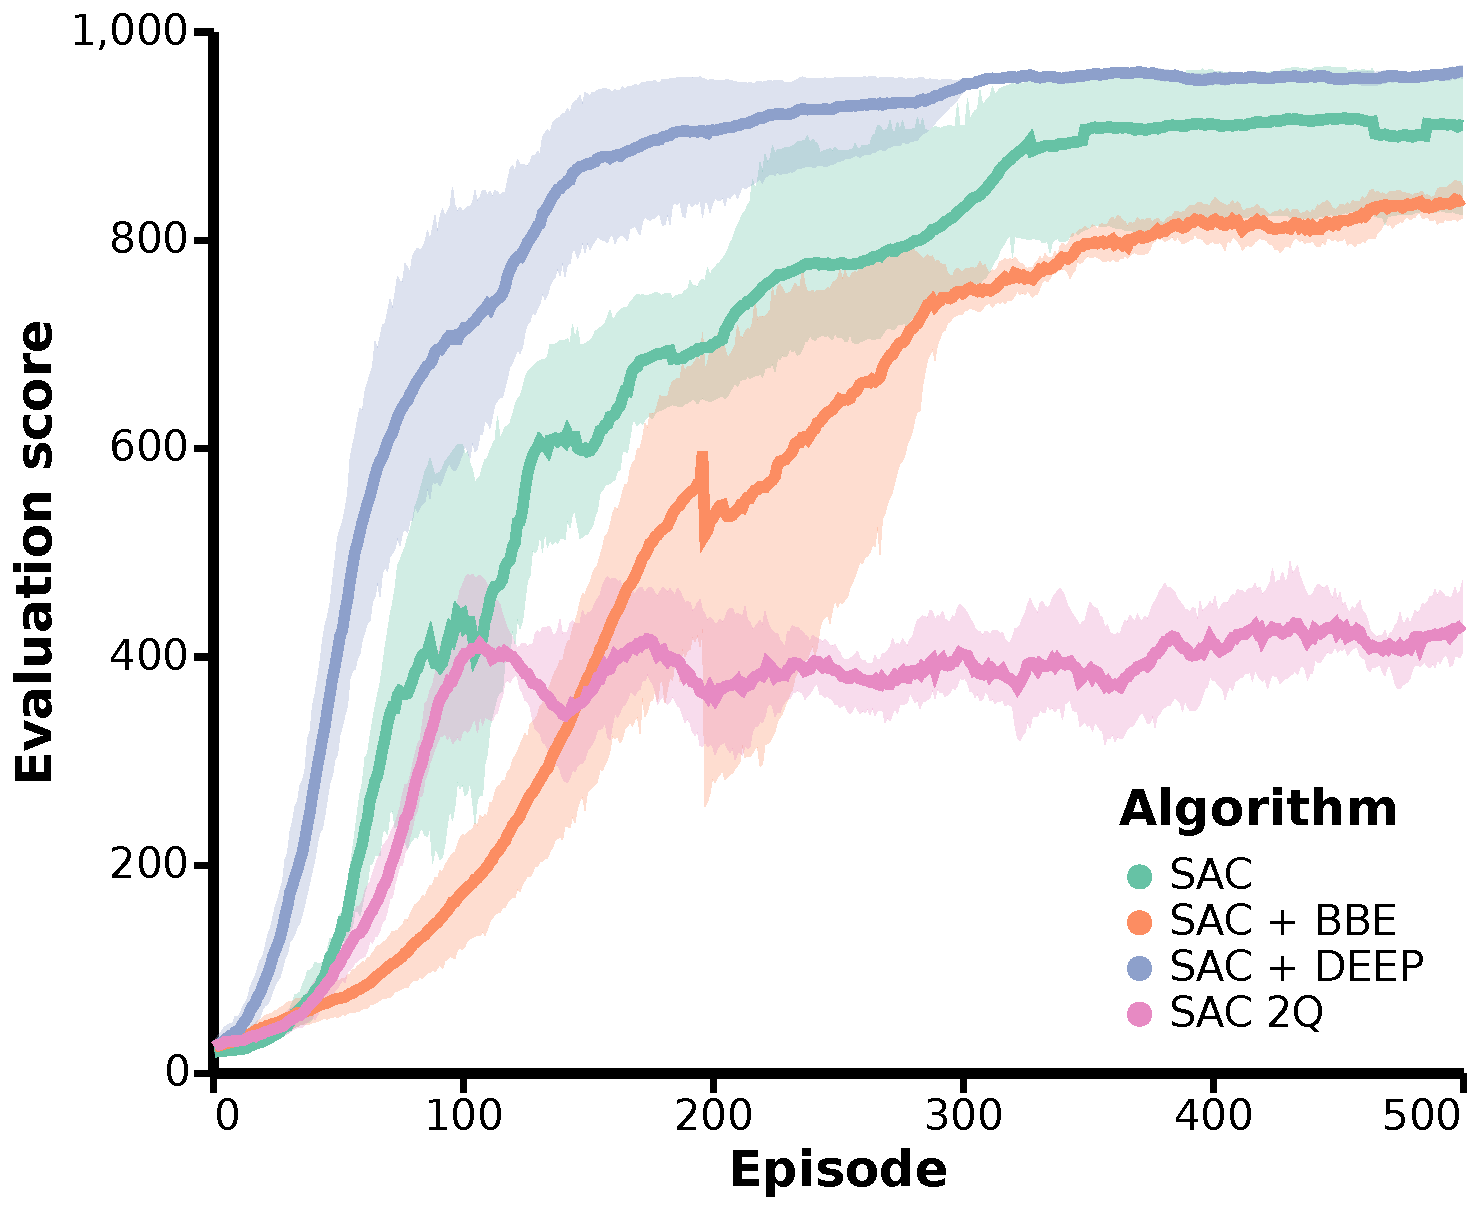
\includegraphics[width=\textwidth]{figures/deep/neurips_SAC2Q_walker_explore.pdf}
        \caption{Walker explore}
    \end{subfigure}
    \caption{SAC 2Q performs uniformly worse than SAC + BBE.}
\end{figure}
% \end{subappendices}
\printendnotes
